\chapter*{Oversikt og repetisjon}
\addcontentsline{toc}{chapter}{Oversikt og repetisjon}
\label{chap:Intro}
Innholdet i dette notatet er standard materiale i ingeniørmatematikken og det finnes mange kilder på nett hvor materialet presenteres på lignende, om enn litt forskjellige, måter. 

\paragraph{Støtteliteratur for Modul 1 og 2: }I de to første delene av kurset (integrasjon og vektorkalkulus) kan vi anbefale følgende:
\begin{itemize}
 \item Standardlærebøker som for eksempel \cite{Adams,K93,MaT88,Furlan}
 \item Forskjellige notater på nett \cite{PON} eller \cite[Kapittel 15 og 16]{SaH}, \cite{MLon}.
 \item Grunnleggende Python finnes for eksempel i \cite{Ch23}.
\end{itemize} 
\paragraph{Støtteliteratur for Modul 3: } For den delen av kurset som omhandler PDEer kan følgende literaturliste være av nytte:
\begin{itemize}
\item Introduksjon, grunnleggende PDEer og bevaringslover: \cite{Deb12,Furlan,Ep17,LaT03}.
\item Grunnleggende numerikk for PDEer: \cite{KaM20}.
\item For endelig-volum-metode kan vi anbefale \cite{VaM07}.
\item Python og Jupyter for numerikk med PDEer finnes for eksempel i \cite{cfd12}.
\end{itemize}




\newpage
\section*{Repetisjon}
I første forelesning skal vi kort repetere matematikken fra tidligere kurs. Blant annet: Notasjon, kontinuitet av funksjoner, vektorregning, partiellderivasjon og integrasjon i én variabel. Dette er områder vi trenger å friske opp i før vi begynner på nytt stoff, så det er viktig at du tar denne repetisjonsjobben på alvor i den grad du har glemt ting.

\subsection*{$\R^n$ og notasjon for vektorer}
Vektorer blir en sentral del av dette faget, og det er viktig å ha en velfungerende notasjon. I og med at vektorer opptrer i mange sammenhenger, slik som både i funksjonsanalyse og i lineær algebra, kan man bli litt forvirret. Så la oss starte med å kjapt repetere og definere grunnleggende vektornotasjon.

For et naturlig tall $n \in \N$ (hvor $\N = \{1,2,3,\ldots\}$) definererer vi det $n$-dimensjonale reelle vektorrommet
\[\R^n = \{(v_1,\ldots, v_n) \colon v_1,\ldots, v_n \in \R\}\]
Vanligvis skriver vi $\vect{v},\vect{w},\ldots$ for vektorer og $\vect{F}, \vect{f}, \ldots$ for funksjoner som har verdier i $\R^n,\ n>1$. Dersom $n=1$ dropper vi gjerne fet skrift for funksjoner og skriver som før $F$, $f$... . Av plasshensyn vil vi som regel skrive vektorer som radvektorer. Men noen ganger er det likevel hensiktsmessig å benytte kolonnevektorer, slik som ved matrisemultiplikasjon. Heldigvis er det lett å transformere den ene til den andre via transponerte.

\begin{defn}{Transponering av matriser}
Vi kommer til å benytte transponering av matriser (med mindre vi glemmer det...) og skriver
\[(x_1, \ldots, x_n)^\top := \begin{bmatrix} x_1 \\ \vdots \\  x_n\end{bmatrix}\]
\end{defn}
Matriseregning antas kjent fra tidligere kurs, men i det følgende repeterer vi likevel noe av det mest grunnleggende.

Vi skal hovedsakelig jobbe med to og tre-dimensjonale vektorrom $\R^2$ og $\R^3$. Det er praktisk å ha en notasjon for de tilhørende standard (kartesiske) basisvektorene i disse rommene.

\begin{defn}{Standardbasis}
For det todimensjonale rommet $\R^2$ skriver vi 
\[\vect{i} = \begin{bmatrix} 1\\ 0\end{bmatrix} \quad ,\quad\vect{j} = \begin{bmatrix} 0 \\ 1\end{bmatrix}.\]
For det tredimensjonale rommet $\R^3$ skriver vi $\vect{i},\vect{j}, \vect{k}$ for de tre enhetsvektorene som danner standardbasis til $\R^3$:
\[\vect{i} = \begin{bmatrix} 1\\ 0\\0\end{bmatrix} \quad ,\quad\vect{j} = \begin{bmatrix} 0 \\ 1\\0\end{bmatrix} \quad ,\quad\vect{k} = \begin{bmatrix} 0 \\ 0\\1\end{bmatrix}.\]
\end{defn}


\subsection*{Operasjoner med vektorer}

Vi minner også om skalarprodukt (prikkprodukt) og vektorprodukt (kryssprodukt). 

\begin{defn}{Skalarprodukt, Prikkprodukt}
For $\vect{v}=(v_1,\ldots, v_n)^\top$, $\vect{w}=(w_1,\ldots w_n)^\top$ 
\[\vect{v} \cdot \vect{w}=\sum_{i=1}^n v_iw_i\]
\end{defn}

Den geometriske fortolkningen av skalaproduktet er også viktig,
dvs. $$\vect{u}\cdot \vect{v} = \cos(\alpha)\cdot |\vect{u}|\cdot |\vect{v}|$$ hvor $\alpha$ er vinkelen mellom vektorene og $|u|$ 
er lengden til vektoren $u$.


For å skrive ned kryssproduktet er det kjekt å først repetere hvordan man beregner determinanten til en kvadratisk matrise. Vi skriver
\[A=\begin{bmatrix} a_{11} & \cdots & a_{1n} \\ \vdots & \ddots & \vdots \\ a_{n1} & \cdots & a_{nn}\end{bmatrix} \qquad \text{det} A = \begin{vmatrix} a_{11} & \cdots & a_{1n} \\ \vdots & \ddots & \vdots \\ a_{n1} & \cdots & a_{nn}\end{vmatrix}\]
Husk at $2\times 2$-matriser har en enkelt formel for determinanten
\[\begin{vmatrix} a & b \\ c & d\end{vmatrix} = ad-bc\]
og for $3\times 3$-matriser kan vi regne ved hjelp av Sarrus-regel som er grafisk fremstilt i neste formel. Her betyr en rød pil at vi multipliserer og adderer elementene og en blå at vi multipliserer men subtraherer:
\NiceMatrixOptions
  { pgf-node-code = \pgfsetfillcolor{white} \pgfusepathqfill }
\pgfset{nicematrix/cell-node/.append style = { inner sep = 1pt } }
\[\begin{NiceArray}{|ccc|>{\color{gray}}c>{\color{gray}}c}
\CodeBefore [create-cell-nodes]
    \begin{tikzpicture} [shorten < = 2pt,shorten > = 2pt]
    \draw [red,->] (1-1) -- (3-3) ;
    \draw [red,->] (1-2) -- (3-4) ;
    \draw [red,->] (1-3) -- (3-5) ;
    \draw [blue,->] (3-1) -- (1-3) ;
    \draw [blue,->] (3-2) -- (1-4) ;
    \draw [blue,->] (3-3) -- (1-5) ;
    \end{tikzpicture}
\Body
    a_{11} & a_{12} & a_{13} & a_{11} & a_{12} \\[2mm]
    a_{21} & a_{22} & a_{23} & a_{21} & a_{22} \\[2mm]
    a_{31} & a_{32} & a_{33} & a_{31} & a_{32} \\
\end{NiceArray}
\]

\begin{defn}{Vektorprodukt}
For to vektorer $\vect{a}=(a_1,a_2,a_3)^\top,\vect{b}=(b_1,b_2,b_3)^\top$ kan vi lage vektorprodukt
\[\vect{a} \times \vect{b} = \begin{vmatrix}\vect{i} & \vect{j} & \vect{k} \\ a_1 & a_2 & a_3 \\ b_1 & b_2 & b_3 \end{vmatrix}\]
\end{defn}

Den geometriske tolkningen av vektorproduktet er også viktig, dvs.
$\vect{u}\times \vect{v}$ står ortogonalt på $\vect{u}$ og $\vect{v}$  
med retning bestemt av høyrehåndsregelen, og
$$|\vect{u}\times\vect{v}| = \sin(\alpha)\cdot |\vect{u}|\cdot|\vect{v}|$$
hvor $\alpha$ er vinkelen mellom vektorene.

Vektorprodukt er egentlig kun definert for $\mathbb{R}^3$. For 
$\mathbb{R}^2$ så kan vi likevel bruke vektorprodukt ved å tenke 
på en to-dimensjonal vektor $(a,b)^\top$ som en vektor i tre 
dimensjoner $(a,b,0)^\top$. Siden produktet da ligger langs
$z$-aksen så er det bestemt av ett tall.



\subsection*{Kontinuerlige funksjoner}
Når man skal behandle deriverte, er det viktig å etablere kontinuitet. For flervariable funksjoner så blir dette litt mer komplisert enn for én-variable funksjoner, ettersom man kan nærme seg et punkt fra flere retninger.

\begin{defn}{Kontinuitet av funksjoner på $\R^n$}{}
La $f(\vect{x})$ være en funksjon av $n$ variable ($n\in\N$), hvor  $\vect{x}=(x_1,...,x_n)$. Vi sier at $f(\vect{x})$ er \textit{kontinuerlig} i punktet $\vect{a}$ dersom 

\[
\lim_{\mathbf{x} \to \mathbf{a}} f(\mathbf{x}) = f(\mathbf{a}).
\]
Mer presist: \(f\) er kontinuerlig i \(\mathbf{a}\) hvis for alle \(\epsilon > 0\) finnes det et \(\delta > 0\) slik at

\[
\|\mathbf{x} - \mathbf{a}\| < \delta \implies |f(\mathbf{x}) - f(\mathbf{a})| < \epsilon.
\]    
\end{defn}
Når man snakker om kontinuitet i flervariabel analyse, kreves det at grenseverdien må eksistere uansett hvilken vei \( \mathbf{x} \) nærmer seg \( \mathbf{a} \). Det vil si: Man kan nærme seg \( \mathbf{a} \) fra uendelig mange retninger og baner (linjer, kurver, spiraler osv.). Hvis det finnes bare én vei der grensen ikke stemmer, så er funksjonen ikke kontinuerlig i det punktet. La oss se på et eksempel.

\begin{eks}{Sjekk av kontinuitet}{}
La oss se på funksjonen:
\[
f(x, y) = 
\begin{cases}
\frac{2xy}{x^2 + y^2}, & (x, y) \neq (0, 0) \\
0, & (x, y) = (0, 0)
\end{cases}
\]

Vi undersøker grenseverdien mot punktet \( (0, 0) \) langs ulike retninger:

\begin{itemize}
    \item Langs linjen \( y = x \):
    \[
    f(x, x) = \frac{2x^2}{2x^2} = 1
    \]
    \item Langs linjen \( y = 0 \):
    \[
    f(x, 0) = 0
    \]
\end{itemize}

Grenseverdien avhenger av retningen man nærmer seg langs, så grensen eksisterer ikke, og funksjonen er \textbf{ikke kontinuerlig} i \( (0, 0) \).
\end{eks}

\begin{rem}{}{}
Å studere grenseverdier langs spesifikke retninger (f.eks. \( x \)-aksen, \( y \)-aksen, eller \( y = x \)) kan brukes til å \emph{falsifisere} kontinuitet. Hvis to ulike retninger gir ulike grenseverdier, er funksjonen ikke kontinuerlig.
\textbf{Men}: Å ha samme grense langs mange retninger er ikke nok til å konkludere med kontinuitet – man må vise at grensen er den samme for \emph{alle} baner inn mot punktet.
\end{rem}

\subsection*{Partiellderiverte}
For en funksjon av flere variabler $f(x,y,z,\ldots)$ skriver vi 
\[\frac{\partial f}{\partial x} , \frac{\partial f}{\partial y} , \frac{\partial f}{\partial z} , \ldots\]
for de partiellderiverte. Ofte skal vi også bruke notasjonen kjent fra fysikk eller differensiallikninger hvor \[f_x := \frac{\partial f}{\partial x} , f_y := \frac{\partial f}{\partial y}, \ldots\]

I tillegg så minner vi om at en flervariabelfunksjon (i motsetning til en envariabelfunksjon) ikke nødvendigvis er deriverbar, selv om 
den har partiellderiverte.  

De aller aller fleste funksjonene vi bruker vil være kontinuerlige og deriverbare, slik at
vi ofte lar være å presisere dette. Vi antar at derivasjonsregler er kjent fra tidligere kurs.

\subsection*{Parametrisering av linjestykker}
Vi kommer også til å parametrisere aktivt i dette kurset. Spesielt skal vi lære å parametrisere kurver og flater. Det kan derfor være kjekt med en aldri så liten oppfriskning av parametrisering av linjestykker. Her ser vi kun på det aller enkleste tilfellet, nemlig et \emph{rett} linjestykke -- mer generelle kurver kommer vi tilbake til senere i kompendiet.

Å \emph{parametrisere} en mengde med punkter vil si å beskrive punktene som verdiene til en funksjon av én (eller flere) parametre. For et linjestykke mellom to punkter $P$ og $Q$ med stedvektorer $\vect{p}$ og $\vect{q}$, er ideen at vi lar en parameter $t$ ``gli'' fra $0$ til $1$, og for hver verdi av $t$ regner vi oss frem til ett punkt langs linjestykket:

\begin{defn}{Parametrisering av et linjestykke}
La $P$ og $Q$ være to punkter med stedvektorer $\vect{p}$ og $\vect{q}$. Linjestykket fra $P$ til $Q$ parametriseres ved
\[
\vect{r}(t) = \vect{p} + t\,(\vect{q}-\vect{p}), \qquad t\in[0,1].
\]
\end{defn}

Legg merke til at $\vect{d}:=\vect{q}-\vect{p}$ er en retningsvektor for linjen (den peker fra $P$ mot $Q$), slik at vi også kan skrive parametriseringen som
\[
\vect{r}(t) = \vect{p} + t\,\vect{d}.
\]
Dette er den samme punkt-retning-formen vi kjenner fra linjelikninger fra før, bare skrevet med en parameter $t$ i stedet for at $y$ uttrykkes direkte som funksjon av $x$ -- en stor fordel, siden denne formen også fungerer for loddrette linjestykker, og for linjestykker i flere dimensjoner.

Vi ser lett at
\begin{itemize}
\item $\vect{r}(0) = \vect{p}$, altså startpunktet $P$,
\item $\vect{r}(1) = \vect{p}+(\vect{q}-\vect{p}) = \vect{q}$, altså sluttpunktet $Q$,
\item for $t\in(0,1)$ får vi punkter som ligger \emph{mellom} $P$ og $Q$ (lineær interpolasjon).
\end{itemize}
Dersom vi i stedet lar $t$ variere over hele $\R$, parametriserer vi hele den \emph{uendelige} rette linjen gjennom $P$ og $Q$, ikke bare linjestykket mellom dem.

La oss se på et konkret eksempel.

\begin{eks}{Parametrisering av et linjestykke}\label{eks:param-linje}
La $P=(1,1)$ og $Q=(5,4)$. Vi ønsker å parametrisere linjestykket fra $P$ til $Q$.

\begin{center}
\begin{tikzpicture}
  \begin{axis}[
    axis lines = middle,
    axis equal image,
    xlabel = {$x$}, ylabel = {$y$},
    xmin=-1, xmax=6.4, ymin=-1, ymax=5.2,
    xtick={1,2,3,4,5}, ytick={1,2,3,4},
    width=8cm,
    enlargelimits=false,
  ]
    \addplot[thick, blue, -latex] coordinates {(1,1) (5,4)};
    \addplot[mark=*, mark size=1.6pt, color=black, forget plot] coordinates {(1,1)};
    \addplot[mark=*, mark size=1.6pt, color=black, forget plot] coordinates {(5,4)};
    \addplot[mark=*, mark size=1.3pt, color=gray, forget plot] coordinates {(3,2.5)};
    \node[below right, font=\footnotesize] at (axis cs:1,1) {$P$, $t=0$};
    \node[above left, font=\footnotesize] at (axis cs:5,4) {$Q$, $t=1$};
    \node[above, font=\footnotesize] at (axis cs:3,2.5) {$t=\tfrac12$};
  \end{axis}
\end{tikzpicture}
\captionof{figure}{Linjestykket fra $P=(1,1)$ til $Q=(5,4)$, parametrisert ved $\vect{r}(t)=(1+4t,\,1+3t)$. Den grå prikken viser punktet ved $t=\tfrac12$.}
\label{fig:param_linje}
\end{center}

\textbf{Steg 1: Finn retningsvektoren.}
\[
\vect{d} = \vect{q}-\vect{p} = (5,4)-(1,1) = (4,3).
\]

\textbf{Steg 2: Sett opp parametriseringen.} Med $\vect{p}=(1,1)$ og $\vect{d}=(4,3)$ gir formelen fra definisjonen over
\[
\vect{r}(t) = (1,1) + t\,(4,3) = (1+4t,\ 1+3t), \qquad t\in[0,1],
\]
altså komponentvis $x(t)=1+4t$ og $y(t)=1+3t$ (se figur~\ref{fig:param_linje}).

\textbf{Steg 3: Kontroller endepunktene.}
\[
\vect{r}(0) = (1,1) = P, \qquad \vect{r}(1) = (1+4,\ 1+3) = (5,4) = Q. \ \checkmark
\]

\textbf{Steg 4: Et punkt underveis.} Setter vi inn $t=\tfrac12$ får vi midtpunktet av linjestykket:
\[
\vect{r}\!\left(\tfrac12\right) = \left(1+4\cdot\tfrac12,\ 1+3\cdot\tfrac12\right) = (3,\ 2.5),
\]
som stemmer med at midtpunktet mellom to punkter er gjennomsnittet av koordinatene deres: $\tfrac12\big((1,1)+(5,4)\big) = (3,2.5)$.
\end{eks}

\subsection*{Tangenter og normaler}

Anta at $f$ er deriverbar i punktet $x_0$. Fra tidligere kurs vet vi at den deriverte $f'(x_0)$ er stigningstallet til \emph{tangentlinjen} til grafen $y=f(x)$ i punktet $(x_0,f(x_0))$. Siden tangentlinjen går gjennom $(x_0,f(x_0))$ med dette stigningstallet, kan vi skrive den på punkt-stigningstall-form:

\begin{defn}{Tangentlinjen til $y=f(x)$ i $x=x_0$}
Dersom $f$ er deriverbar i $x_0$, er tangentlinjen til grafen $y=f(x)$ i punktet $(x_0,f(x_0))$ gitt ved
\[
y = f(x_0) + f'(x_0)\,(x-x_0).
\]
\end{defn}

En retningsvektor for tangentlinjen er $\vect{t} = (1,\, f'(x_0))^\top$: dersom $x$ øker med $1$, øker $y$ langs tangenten med nettopp $f'(x_0)$.

\emph{Normallinjen} til kurven i samme punkt står vinkelrett på tangentlinjen, og her kommer skalarproduktet til nytte: to vektorer $\vect{v}$ og $\vect{w}$ står vinkelrett på hverandre nøyaktig når $\vect{v}\cdot\vect{w}=0$. Vi leter derfor etter en retningsvektor $\vect{n}=(a,b)^\top$ for normallinjen som oppfyller
\[
\vect{t}\cdot\vect{n} = 1\cdot a + f'(x_0)\cdot b = 0.
\]
Velger vi for eksempel $b=1$, gir dette $a = -f'(x_0)$, altså $\vect{n} = (-f'(x_0),\,1)^\top$. Stigningstallet til normallinjen blir dermed $b/a = -1/f'(x_0)$ (forutsatt $f'(x_0)\neq 0$), og normallinjen kan skrives
\[
y = f(x_0) - \frac{1}{f'(x_0)}\,(x-x_0).
\]

La oss se på et konkret eksempel hvor vi også tegner opp situasjonen.

\begin{eks}{Tangent og normal til et tredjegradspolynom}\label{eks:tangent-normal-kubikk}
La $f(x) = x^3 - x$, og se på punktet der $x_0 = 1$. Vi ønsker å finne tangentlinjen og normallinjen til grafen $y=f(x)$ i dette punktet.

\begin{center}
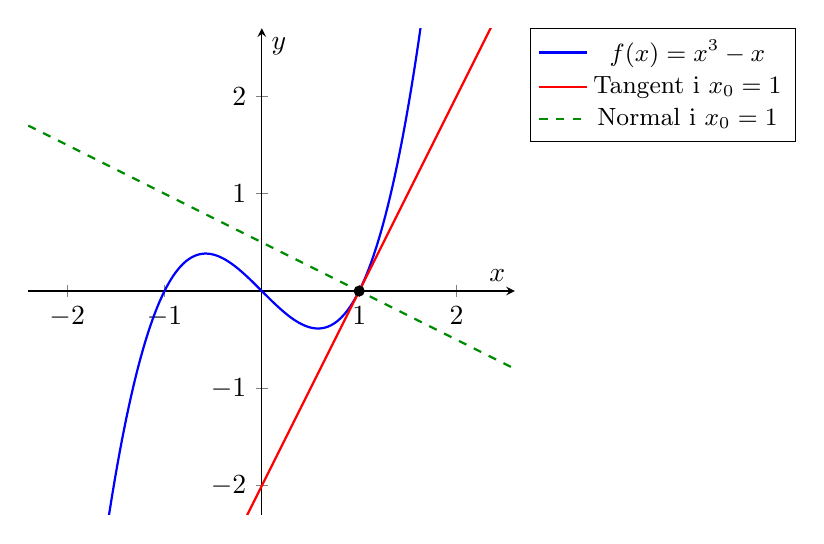
\begin{tikzpicture}
  \begin{axis}[
    axis lines = middle,
    axis equal image,
    xlabel = {$x$}, ylabel = {$y$},
    xmin=-2.4, xmax=2.6, ymin=-2.3, ymax=2.7,
    xtick={-2,-1,1,2}, ytick={-2,-1,1,2},
    width=9cm,
    legend pos=outer north east,
    legend style={font=\small},
    enlargelimits=false,
  ]
    \addplot[domain=-1.8:1.8, samples=150, thick, blue] {x^3-x};
    \addlegendentry{$f(x)=x^3-x$}
    \addplot[domain=-2.4:2.6, samples=2, thick, red] {2*x-2};
    \addlegendentry{Tangent i $x_0=1$}
    \addplot[domain=-2.4:2.6, samples=2, thick, green!55!black, dashed] {-0.5*x+0.5};
    \addlegendentry{Normal i $x_0=1$}
    \addplot[mark=*, mark size=1.8pt, color=black, forget plot] coordinates {(1,0)};
  \end{axis}
\end{tikzpicture}
\captionof{figure}{Grafen til $f(x)=x^3-x$ med tangentlinjen (rød) og normallinjen (grønn, stiplet) i punktet $P=(x_0,f(x_0))=(1,0)$ (markert med en prikk).}
\label{fig:tangent_normal_kubikk}
\end{center}

\textbf{Steg 1: Finn punktet.} Vi setter $x_0=1$ inn i $f$:
\[
f(1) = 1^3 - 1 = 0,
\]
så tangeringspunktet er $(x_0,f(x_0)) = (1,0)$ (se figur~\ref{fig:tangent_normal_kubikk}).

\textbf{Steg 2: Deriver.} Den deriverte er
\[
f'(x) = 3x^2 - 1 \quad\Longrightarrow\quad f'(1) = 3\cdot 1^2 - 1 = 2.
\]

\textbf{Steg 3: Sett opp tangentlinjen.} Med punktet $(1,0)$ og stigningstall $f'(1)=2$ gir tangentlinjeformelen
\[
y = f(x_0) + f'(x_0)(x-x_0) = 0 + 2(x-1) = 2x-2.
\]
En retningsvektor for tangenten er dermed $\vect{t} = (1,2)^\top$ (rød linje i figuren).

\textbf{Steg 4: Finn normalen ved hjelp av skalarproduktet.} Vi leter etter $\vect{n}=(a,b)^\top$ slik at $\vect{t}\cdot \vect{n}=0$:
\[
\vect{t}\cdot \vect{n} = 1\cdot a + 2\cdot b = 0.
\]
Velger vi $b=1$, gir dette $a=-2$, så $\vect{n} = (-2,1)^\top$ er en retningsvektor for normalen. Stigningstallet til normalen er dermed
\[
\frac{b}{a} = \frac{1}{-2} = -\frac12.
\]
Normallinjen gjennom $(1,0)$ med dette stigningstallet blir
\[
y = 0 - \frac12(x-1) = -\frac12 x + \frac12
\]
(grønn, stiplet linje i figuren). Vi kan enkelt verifisere at tangent- og normalvektoren faktisk står vinkelrett på hverandre:
\[
\vect{t}\cdot\vect{n} = (1)(-2) + (2)(1) = -2+2=0. \ \checkmark
\]
\end{eks}

\subsection*{Nivåkurver}

\subsection*{Integrasjon av énvariabelfunksjoner}
Når det gjelder integrasjon så antar vi at dete er kjent fra foregående kurs. Her er en liste over tema du bør friske opp dersom du har glemt det:
\begin{itemize}
    \item Integrasjon som areal
    \item Definisjon ved hjelp av Riemannsummer (Dette blir repetert
i detalj under tema dobbeltintegrasjon under).
\item Integrasjon av potensfunksjoner, eksponensialfunksjoner, trigonometriske funksjoner, $1/x$.
\item Summer av funksjoner og multiplikasjon med konstanter i integrasjoner.
\item Integrasjon ved substitusjon av variable 
\item Delvis integrasjon.
\end{itemize}




\subsection*{Python}
Når det gjelder Python så antar vi igjen at det mest grunnleggende er kjent. Dette gjelder 
\begin{itemize}
\item Programmene som brukes (f.eks. Anaconda, JupyterHub, VSCode, Spyder e.l.).
\item Grunleggende Pythonprogrammering og bruk av matematikk i Python.
\item Funksjonsdefinisjoner med ``def'' og lambda-definisjon av funksjoner.
\item Bruk av Numpy.
\end{itemize}
Se \cite[Introduction and Appendix]{Ch23} eller \cite{cfd12} for mer informasjon.

